\documentclass[a4paper]{jpconf}
\usepackage{graphicx}
\usepackage{listings}
\begin{document}
\title{Dirac integration with a general purpose bookkeeping DB: a complete general suite for distributed resources exploitation}

\author{M Chrząszcz, C De Santis, G Donvito, A Fella, R Grzymkowski, B Santeramo, L Tommassetti, M Zdybał}
%\address{\textsuperscript {1} Institution, Country}
\ead{bruno.santeramo@ba.infn.it}

%%%%%%%%%%%%%%%%%%%%%%%%%%%%%
% (in drafts/<username> we can place drafts...)
%
% DRAFTS USEFUL TO COMPLETE THIS PAPER
% TO REMOVE BEFORE SUBMISSION
%
%\cleardoublepage 
%\include{drafts/bruno/job_submission}
%\include{drafts/bruno/todo_list}
%\include{drafts/bruno/preparing_test}
%\cleardoublepage 
%%%%%%%%%%%%%%%%%%%%%%%%%%%%%

\begin{abstract}
In the context of High Energy Physics computing field the R\&D studies aimed to
the definition of the data and workload models have been carried on and 
completed by the Super$B$ community beyond the experiment life itself.
The work resulted of great interest for a generic mid- and small size VO to 
fulfill Grid exploiting requirements involving CPU-intensive tasks.

We present the R\&D line achievements in the design, developments and test of a
distributed resource exploitation suite based on DIRAC. The main components of
such a suite are the information system, the job wrapper and the new generation
DIRAC framework. The DB schema and the SQL logic have been designed to be able
to be adaptive with respect to the VO requirements in terms of physics 
application, job environment and bookkeeping parameters. A deep and flexible 
integration with DIRAC features has been obtained using SQLAlchemy technology
allowing mapping and interaction with the information system. A new DIRAC
extension has been developed to include this functionality along with a new set
of DIRAC portal interfaces aimed to the job, distributed resources, and
metadata management. The results of the first functionality and efficiency
tests will be reported.
\end{abstract}

\section{Introduction}

\section{Description of suite design}
% Marcin
philosophy: simple, standard and long term solution\\
bird's eye view all over the project\\
 
\section{The Dirac extension} 
% Rafal
- extension structure description\\
- Dirac general purpose project short description + Dirac configuration\\
- service and systems description in detail\\
- web interface components description\\


\section{Bookkeeping DB integration}
% Milosz -> SQLAlchemy
% Luca, Christian -> SBK
- Software layer based on SQLAlchemy\\
-- advantages using SQLAlchemy: Object relational Mapping, clean code, fast\\
-- development, change of DB backend\\
- BK description, highlighting the general purpose characteristics\\
-- session, request, dataset concept\\

 
\section{Job wrapper component}
% Bruno, Armando
- general workflow\\
- data management policy: stage-in and stage out strategies\\
 
\section{Simulation production use case: the SuperB experience}
% Bruno
- general description: workflow, Dirac portal design\\
- past experience: the webui project\\
-- Session definition interface --> DB dynamic build up\\
 
\section{Test session}
% Bruno
A test session was performed aiming to demonstrate the awareness of SuperBDIRAC to integrate the monitoring of a bookkeeping database in DIRAC.
\subsection{Goal description}
DIRAC capabilities and performance as job management tool are well documented (insert some reference). Super$B$ distributed simulation stack (WebUI + SBK + Severus) was successfully used in 3 simulation campaigns (ask to Armando for confirmation and references).\\
Test goal was to demonstrate SuperBDIRAC is capable of substitute WebUI as monitoring tool for job submission, showing data from a bookkeeping database. Test "Q-factor" was the exact corrispondence of information as stored in SBK and displayed in SuperBDIRAC, like in WebUI monitoring page. Correct execution of simulation jobs is not important while the bookkeping information are properly managed.

\subsection{Testbed description}

\begin{figure}[h]
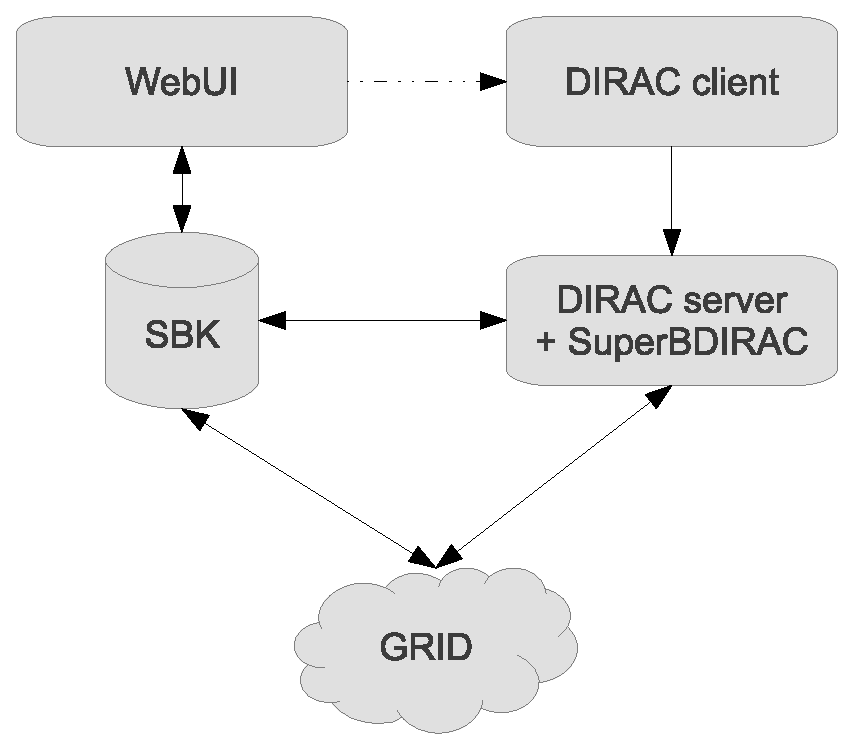
\includegraphics[width=14pc]{img/testbed.eps}\hspace{2pc}%
\begin{minipage}[b]{14pc}\caption{\label{label}Testbed schema.}
\end{minipage}
\end{figure}

FastSim job submission is created via WebUI interface (see figure to be inserted). Once submission is created, a set of scripts and configuration files are created whose path is reported by WebUI interface: in particular the path of php submission script is taken to be be parsed. Since WebUI is still linked with SBK, this portal acts as well as monitoring portal, useful for a check-cross between info displayed in SBK, WebUI and SuperBDIRAC.\\

A python script (mc\_production.py) acts as parser for php submission script and interface with DIRAC client. Once taken all submission parameter, mc\_production.py uses DIRAC API to submit jobs to DIRAC server.\\

DIRAC server receive jobs from DIRAC client, than starts the normal workflow for job management in DIRAC: scheduling, pilot submission, payload retrieval and execution, stageout. Since DIRAC server is equipped with SuperBDIRAC, even bookkeeping monitoring is performed by this component.\\

In SBK the job submission insertion is performed by WebUI, while later info are updated by Severus script executed with every job submitted. Severus interact with SBK via REST interface, while WebUI and SuperBDIRAC have direct acces to SBK since they are in the same LAN area (ask to Armando for confirmation).\\

Jobs were submitted via grid by DIRAC server. Submission was performed using WMS instead of using direct submission to CREAM CE.\\

Submission site was INFN-T1, which ensured CPU time to execute latest simulations related to Super$B$ once the experiment closure.

\subsection{Test description}

Every job simulated 3000 events: this value was chosen to have an execution time of about 10 minutes.
Physical parameters were the same of several official productions.
3 main bunch submission of 400 jobs were performed at INFN-T1 to obtain a total 1200 simulations.
In addition, 2 bunch submission of 10 jobs were performed, again at INFN-T1, to force some failure message in SBK and catch it even in SuperBDIRAC monitoring. In summary, 1220 jobs were submitted for test.\\

Since test goal, several screenshots of WbUI and SuperBDIRAC monitoring were saved, in addition to SBK data screenshots.

\subsection{Results and conclusions}

\section{Conclusions}

- We are offering a Dirac extended suite capable to satisfy the
needs onsmall and mid size VOs in terms of distributed
resource exploitation....

%% \begin{figure}
%% \begin{center}
%% \includegraphics[width=30pc]{schema.pdf}
%% \caption{Dirac suite design schema}
%% \label{fig:superb_sites}
%% \end{center}
%% \end{figure}


\section*{References}
%%%%%%%%%%%%%%%%%%%%%%%%%%%%%%%%%%%%%%%%%%%

\begin{thebibliography}{30}
%% \bibitem{superb}
%% The Super$B$ Collaboration, \emph{SuperB Progress Report, Detector},
%% \verb"http://arxiv.org/abs/1007.4241v1"

%% \bibitem{ref:miur}
%% \verb"http://www.istruzione.it/web/hub/home"

%% \bibitem{ref:babar}
%% Aubert B et al., 2002 {\it Nucl. Instr. Meth. Phys. Res.}, A 479, 1.

%% \bibitem{ref:belle}
%% The Belle Collaboration 2002 The Belle Detector, {\it Nucl. Instrum. Methods Phys. Res.}, Sect. A 479, 117.

%% \bibitem{atlas}
%% The ATLAS Collaboration, {\it ATLAS Detector and Physics Performance Technical Design
%% Report}, http://atlas.web.cern.ch/Atlas/GROUPS/PHYSICS/TDR/access.html.

%% \bibitem{cms}
%% The CMS Collaboration, {\it CMS Detector Technical Design Report}, http://cmsdoc.cern.ch/cms/cpt/tdr/.

%% \bibitem{ref:chep_dist}
%% Bianchi F, Brown D, Corvo M, Di Simone A, Fella A, Gianoli A, Luppi E, 
%% Morandin M, Paoloni E, Rama M, Tomassetti L 2010 {\it Computing for the Next
%% Generation Flavour Factories}, Proceeding of conference CHEP 2010, Computing for
%% High Energy Physics, Taipei, Taiwan, 18-22 October 2010

%% \bibitem{ref:fast_ieee}
%% Andreassen R et al 2010 {\it FastSim: fast simulation of the SuperB detector},
%% Proceeding of conference IEEE NSS-MIC 2010, Knoxville, TN, USA

%% \bibitem{ref:fast_sim}
%% Di Simone A, Gaponenko I, Manoni E, Perez A, Rama M, Roberts D, 
%% Rotondo M, Simi G, Sokoloff M, Suzuki A, Walsh J 2010 {\it FastSim: fast
%% simulation of the SuperB detector}, Proceeding of conference IEEE NSS-MIC
%% 2010,
%% Knoxville, TN, USA

%% %\bibitem{ref:chep_prod} 
%% %D. Brown, M. Corvo, A. Di Simone, A. Fella, E. Luppi, E. Paoloni, R. Stroili, L.
%% %Tomassetti, \emph{The Distributed Production System of the Super$B$ Project:
%% %Description and Results}. Proceeding of conference CHEP 2010, Computing for High
%% %Energy Physics, Taipei, Taiwan, 18-22 October 2010

%% \bibitem{ref:ieee_prod}
%% Brown D, Corvo M, Di Simone A, Fella A, Luppi E, Paoloni E, Stroili R and Tomassetti L 2010 {\it First Results from the SuperB Simulation Production System}. Proceeding of conference IEEE 2010, NSS-MIC 
%% 2010, Knoxville, TN, USA

%% \bibitem{ref:babar_cm}
%% Bozzi C, Adye T, Andreotti D, Antonioli E, Barlow R, Bense B, Boutigny D, Brew C A J, Colling D, Cowles R D, Elmer P, Feltresi E, Forti A, Grosdidier G, Hasan A,  Lacker H, Luppi E, Martyniak J, McNab A, Petzold A, Smith D A, Sundermann J E and Veronesi P 2003 {\it Using the Grid for the BaBar Experiment}, Nuclear Science Symposium Conference Record, 2003 IEEE, 1626 - 1629 Vol.3

%% %N. Geddes \emph{The BaBar Computing Model}. SLAC-PUB-9964, April 1994

%% \bibitem{egi} 
%% \verb"http://www.egi.eu"

%% \bibitem{osg} 
%% \verb"http://www.opensciencegrid.org"

%% \bibitem{dirac} 
%% \verb"http://diracgrid.org"

%% %\bibitem{ref:nordugrid} 
%% %\verb"http://www.norduGrid.org"

%% \bibitem{ref:westgrid} 
%% \verb"http://www.westgrid.ca"

%% \bibitem{ref:lcg-tdr} 
%% The LCG TDR Editorial Board 2005 {\it LHC Computing Grid}, Technical Design
%% Report LCG-TDR-001 CERN-LHCC-2005-024

%% \bibitem{ref:ganga}
%% \verb"http://ganga.web.cern.ch/ganga"

%% \bibitem{ref:wms}
%% \verb"http://glite.web.cern.ch/glite"

%% \bibitem{ref:voms}
%% \verb"http://hep-project-grid-scg.web.cern.ch/hep-project-grid-scg/voms.html"

%% \bibitem{ref:lfc}
%% \verb"https://twiki.cern.ch/twiki/bin/view/LCG/LfcAdminGuide"

%% \bibitem{lcg}
%% \verb"http://lcg.web.cern.ch/LCG"

%% \bibitem{ref:srm}
%% \verb"http://sdm.lbl.gov/srm-wg/doc/SRM.v2.2.html"

%% \bibitem{ref:storm}
%% Corso A et al. 2006 {\it StoRM, an SRM Implementation for LHC Analysis Farms
%% Computing in High Energy Physics} (CHEP 2006), Mumbai, India, Feb. 13-17

%% \bibitem{ref:dcache}
%% Fuhrmann P and Glzow V, dCache 2006 {\it Storage System for the Future}.
%% New York: Lecture Notes in Computer Science/Springer, vol. 4128, pp.
%% 1106-1113.

%% \bibitem{ref:dpm}
%% \verb"https://twiki.cern.ch/twiki/pub/LCG/DataManagementUsefulPresentations/chep 07\_poster_DPM.ppt"

%% \bibitem{ref:hadoop}
%% \verb"http://hadoop.apache.org/"

\bibitem{ref:rest}
Fielding R T 2000 {\it Architectural Styles and The Design of Network-based
Software Architectures }, PhD Thesis, University of California Irvine

\bibitem{ref:webui}
A.Fella, E.Luppi, L.Tomassetti \emph{A General Purpose Suite for Job Management, Bookkeeping and Grid Submission}. International Journal of Grid Computing \& Applications (IJGCA) Vol.2, No.2, June 2011. DOI: 10.5121/ijgca.2011.2202.

\end{thebibliography}


\end{document}


